%\documentclass[handout]{beamer}
\documentclass{beamer}
\usetheme{default}
\usepackage{hyperref}
\usepackage{listings}
\title{Software Testing \\ Introduction}
\author{Justin Pearson}
\date{2020}
\setbeamertemplate{footline}[page number]
\setbeamertemplate{navigation symbols}{}
\begin{document}
\lstset{language=python}

\begin{frame}
  \maketitle
\end{frame}
\begin{frame}{Distance Teaching 2020}
  \begin{itemize}
  \item   Due to the current Covid-19 situation this course is going to be
  taught online. 
 \item  I plan to flip all the lectures. Links to online videos will
   be posted on the web. I will then  be available for the first hour
   of the scheduled lecture session to answer questions.
 \end{itemize}
 Please look at the course homepage
 \begin{itemize}
 \item \url{http://user.it.uu.se/~justin/Hugo/courses/softwaretesting/}
 \end{itemize}
\end{frame}
\begin{frame}{Course Text Book}
  \begin{itemize}
  \item Introduction to Software Testing" by Paul Amman and Jeff
    Offut. Second Edition. 
  \end{itemize}
  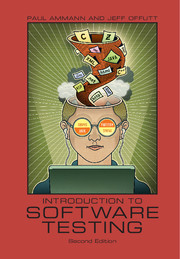
\includegraphics{textbookcover.jpg}
  
\end{frame}
\begin{frame}
  \frametitle{Outline}
  \begin{itemize}
  \item Lectures.
  \item Exercise on Test driven development. Done alone.
  \item Project, groups of 5-6. Test case development for a python
    library of your choice.
  \item Exam
  \end{itemize}
\end{frame}
\begin{frame}{Very brief Overview of the Course}
  \begin{itemize}
  \item Test Driven Development
  \item The limitations of testing
  \item Code coverage. What does it mean and how to achieve it?
  \item Logic based coverage
  \item Input Domain Modelling
  \item Test Oracles and Property Based Testing
  \item Practical Concerns: Test Plans and the role of testing in a
    large software project
  \item Continuous integration and testing 
  \end{itemize}
\end{frame}
\begin{frame}
  \frametitle{Grading}
  \begin{itemize}
  \item The Exam is U,3,4,5
  \item Project work and the lab is pass/fail.
  \end{itemize}
\end{frame}
\begin{frame}
  \frametitle{Lab}
  \begin{itemize}
  \item Test driven development exercise. Using author name parsing in
    BibTex. 
  \end{itemize}
\end{frame}
\begin{frame}
  \frametitle{Project}
  \begin{itemize}
  \item White box and Black box testing for a python library of your choice.
  \item Written report deadline 2021-01-15
  \item You must document what your tests are designed to do.
  \end{itemize}
\end{frame}
%\begin{frame}
%  \frametitle{Lecture slides and revision}
%  \begin{itemize}
%  \item My lecture slides are rather sparse. You will not be able to
%    pass the exam by simply looking at the slides. You will need to
%    read the relevant sections of the book. 
%\item Some of the lab and project work will also prepare you for the
%  exam. From your work on test design and documentation you will
%  prepare yourself to answer some more reflective questions on the exam.
%  \end{itemize}
%\end{frame}
%
\begin{frame}
  \frametitle{What will you learn?}
  \begin{itemize}
  \item Software testing is an interesting mix of art and theory.
    \begin{itemize}
    \item Theory tells you that testing is impossible, but
    \item Testing does improve software quality.
    \end{itemize}
  \item I will give you the tools to develop tests in a more
    principled way. You will be given the theoretical tools to think
    about questions such as:
    \begin{itemize}
    \item What do my tests cover?
    \item What does coverage actually mean? 
    \end{itemize}
  \end{itemize}
\end{frame}
\end{document}

%%% Local Variables:
%%% mode: latex
%%% TeX-master: t
%%% End:
